\section{EVD user interface}
\subsection{Log in}
\begin{figure}[H]
    \centering
    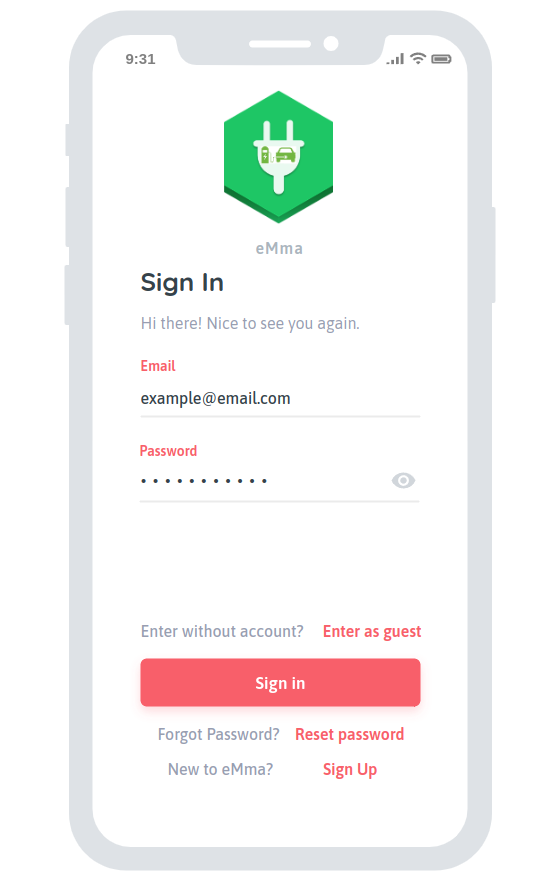
\includegraphics[width=0.4\textwidth]{Images/cp3/logIn.png}
    \caption{UI for the log in}
\end{figure}
We can see from the UI for the log in that the operation is very simple. To sign up is enough to enter the email and the password used during the registration. The EVD can enter into eMma as a guest, if he doesn't want to sign up, but in that case it will perceive only some limited functionalities of the application. It can also be useful to set a mechanism to manage the case in which the user forgets his password.

\subsection{Register}
\begin{figure}[H]
    \centering
    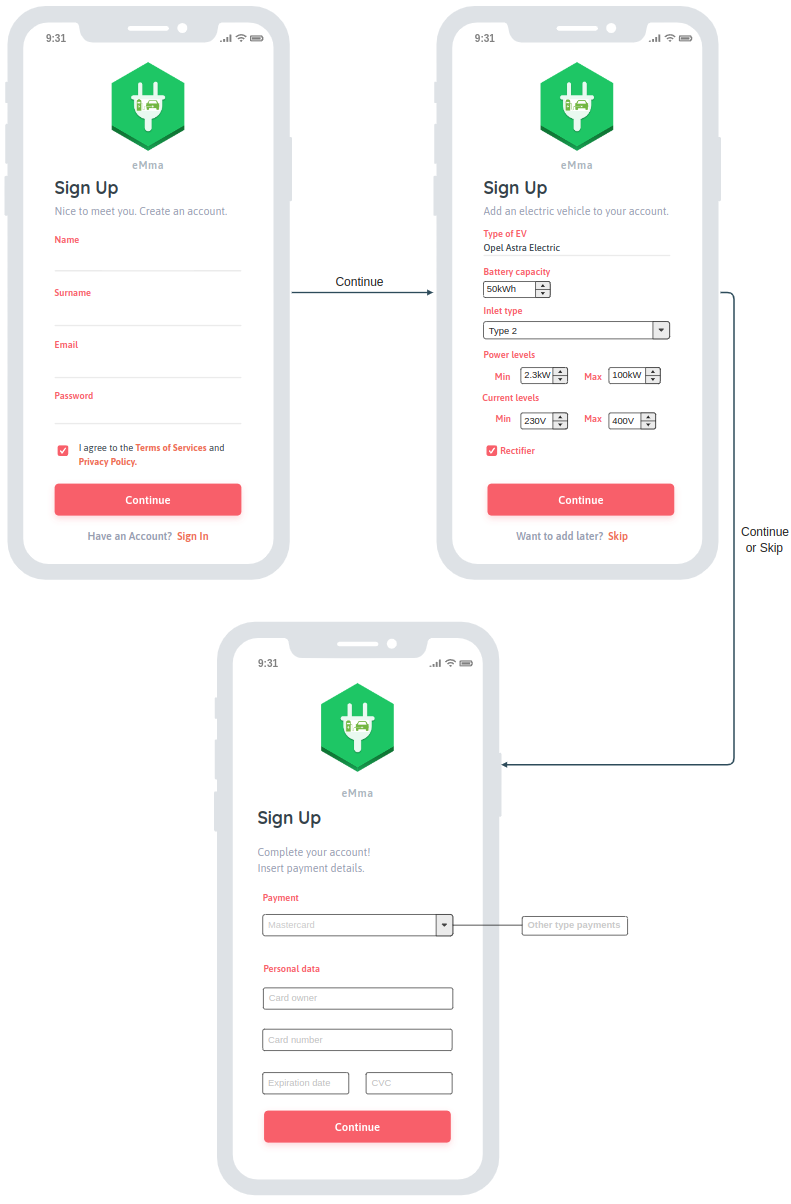
\includegraphics[width=0.85\textwidth]{Images/cp3/registerMockup.png}
    \caption{UI for registration}
\end{figure}
The UI for the registration was thought in order to be as user-friendly as possible. First, to sign up is necessary to insert some personal data, such as the name, the surname, and the email and password that will be used for the log in, as previously explained. It is also necessary to accept the 'Term of Service' in order to continue with the registration. The second step asks the user to add some data about his EV and we can see that the insertion is guided by the interface in order to avoid as much as possible data errors. The EVD has to add the type of the EV, the inlet type, the power levels and the current levels, and has to check or not the final box to inform if the car has or not the rectifier. Finally, to complete the sign up process the user is requested to insert the payment details. After registration, from the personal profile the EVD will be able to add new data to his profile, such as new payment methods and new EVs, and he will be able to modify these ones.

\subsection{Charge now}
\begin{figure}[H]
    \centering
    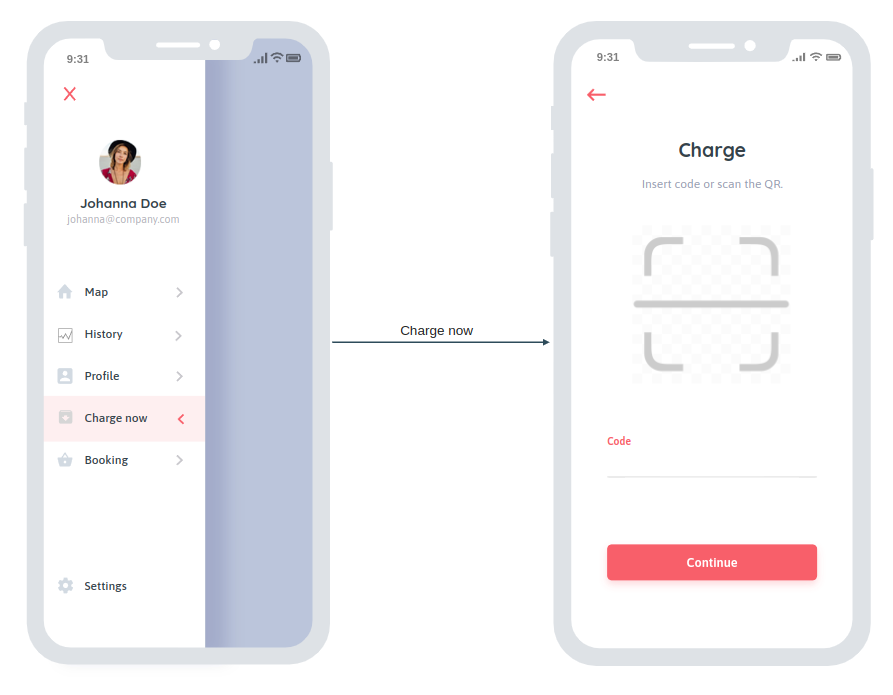
\includegraphics[width=0.85\textwidth]{Images/cp3/chargeNow.png}
    \caption{UI for starting the charging session}
\end{figure}
To start the charging process the EVD has to insert the code or scan the QR present on the charging point. This can be started from the menu or from the 'Charge now' button present in the charging station page, as we will see in the following mock-ups. 

\subsection{Visualize stations}
\begin{figure}[H]
    \centering
    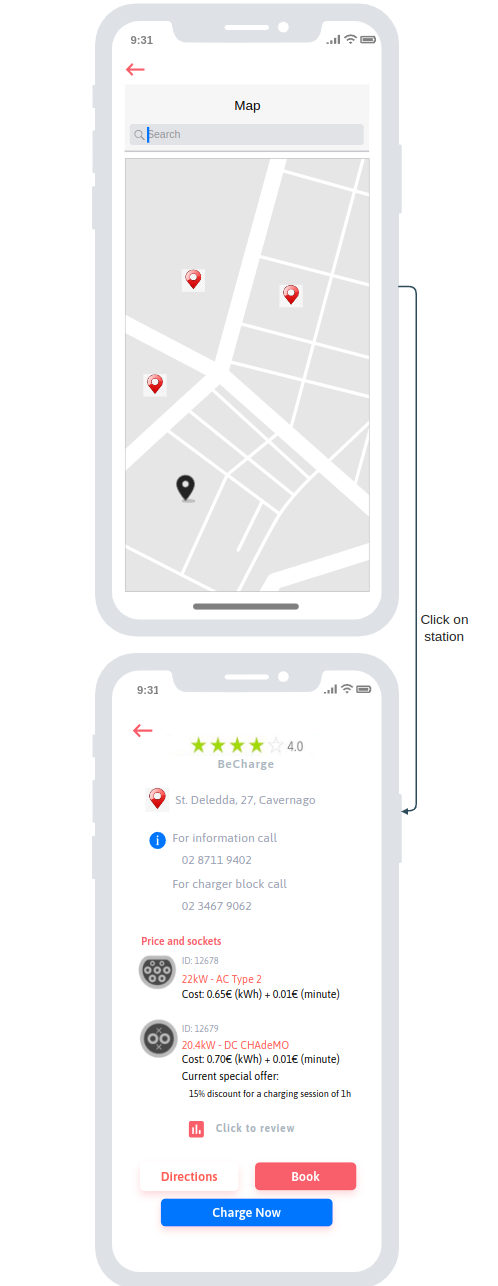
\includegraphics[width=0.4\textwidth]{Images/cp3/visualizeStations.png}
    \caption{UI to visualize stations on the map and their information}
\end{figure}
The main page of the eMma shows to the user the map and permits to visualize the charging stations nearby or to insert a position in which to search for new stations. Clicking on one of the stations, the application shows the charging station page with the most important information: the rating, the name of the station, the address and the contacts, the available sockets and the respective prices and special offers. Finally, it is possible to leave a review or to see the ones left by other users. From this page is possible to get the directions to reach the station and it is also possible to start the main operations of the system: the charging session and the booking of a charging point.

\subsection{Booking charging point}
\begin{figure}[H]
    \centering
    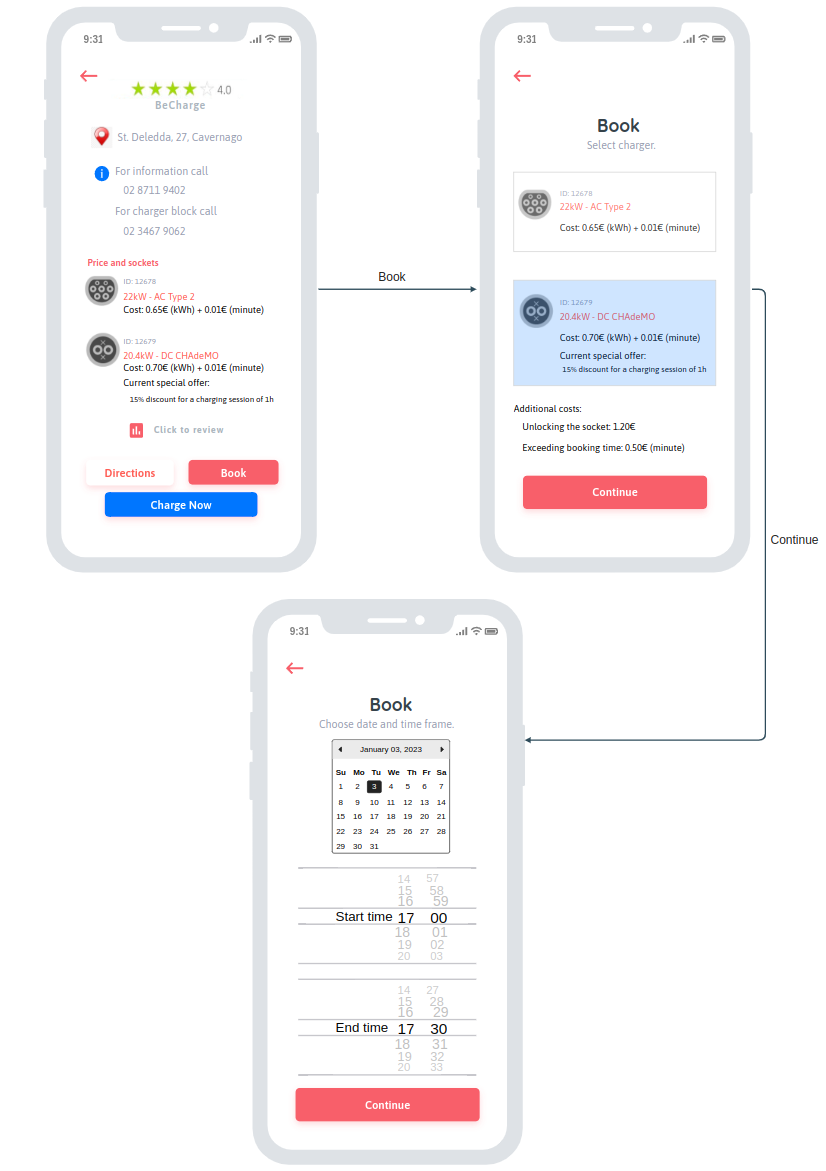
\includegraphics[width=0.75\textwidth]{Images/cp3/bookingCP.png}
    \caption{UI to book the charging point in a certain time frame}
\end{figure}
During the booking operation the EVD has to select the charging point he wants to book from the selected station and also to insert the date and the time frame of the booking. 

\subsection{Terminate charging}
\begin{figure}[H]
    \centering
    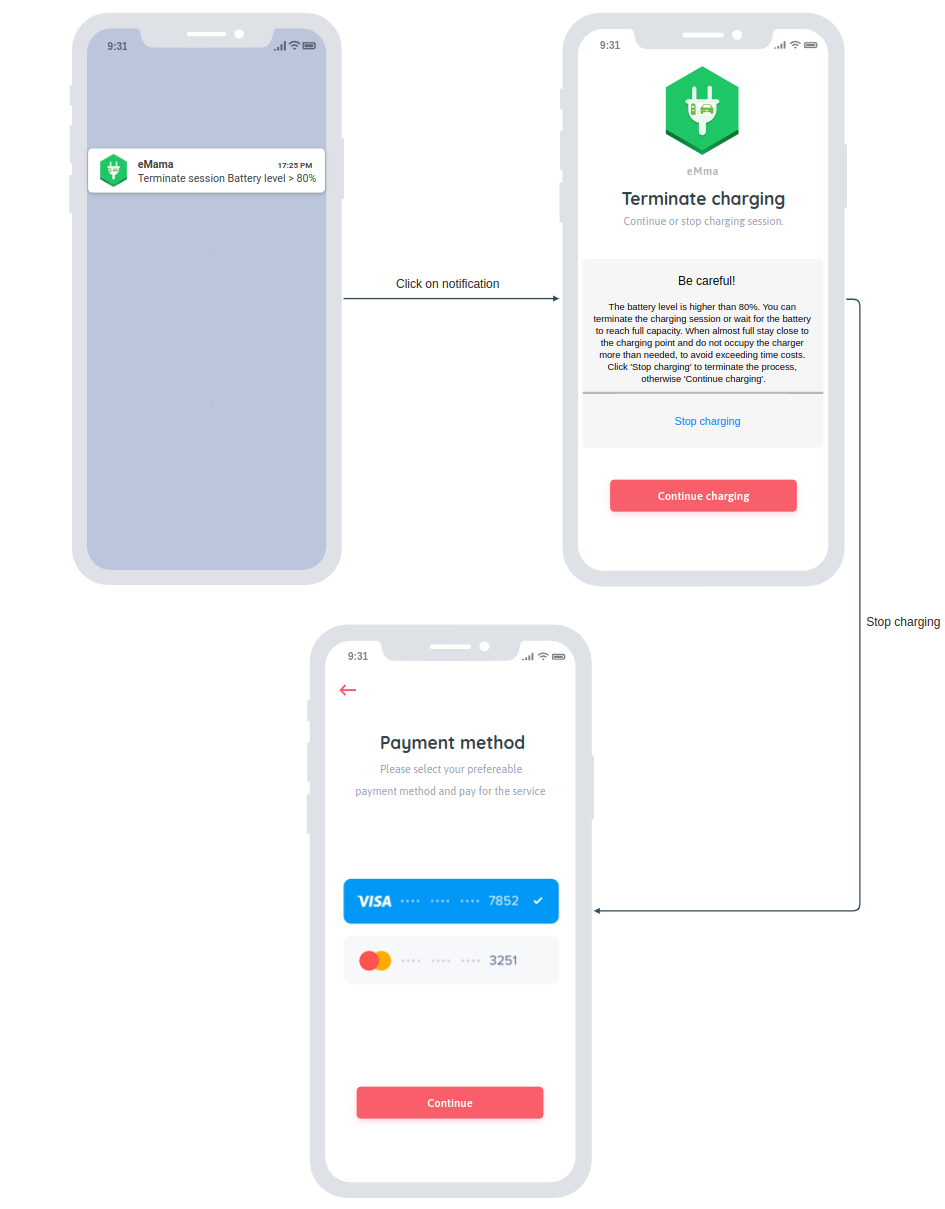
\includegraphics[width=0.9\textwidth]{Images/cp3/terminateCharging.png}
    \caption{UI to terminate the charging session}
\end{figure}
We can see from this UI, that the eMma sends a notification to the user smartphone when the battery level reaches 80\%. The user can decide if he wants to stop the charging session or proceed with the charging until full battery. When the EVD decides to terminate the charging the eMma asks to select the payment method in order to pay for the service.

\clearpage
\section{CPO user interface}
\subsection{Visualize stations and add a general promotion}
\begin{figure}[H]
    \centering
    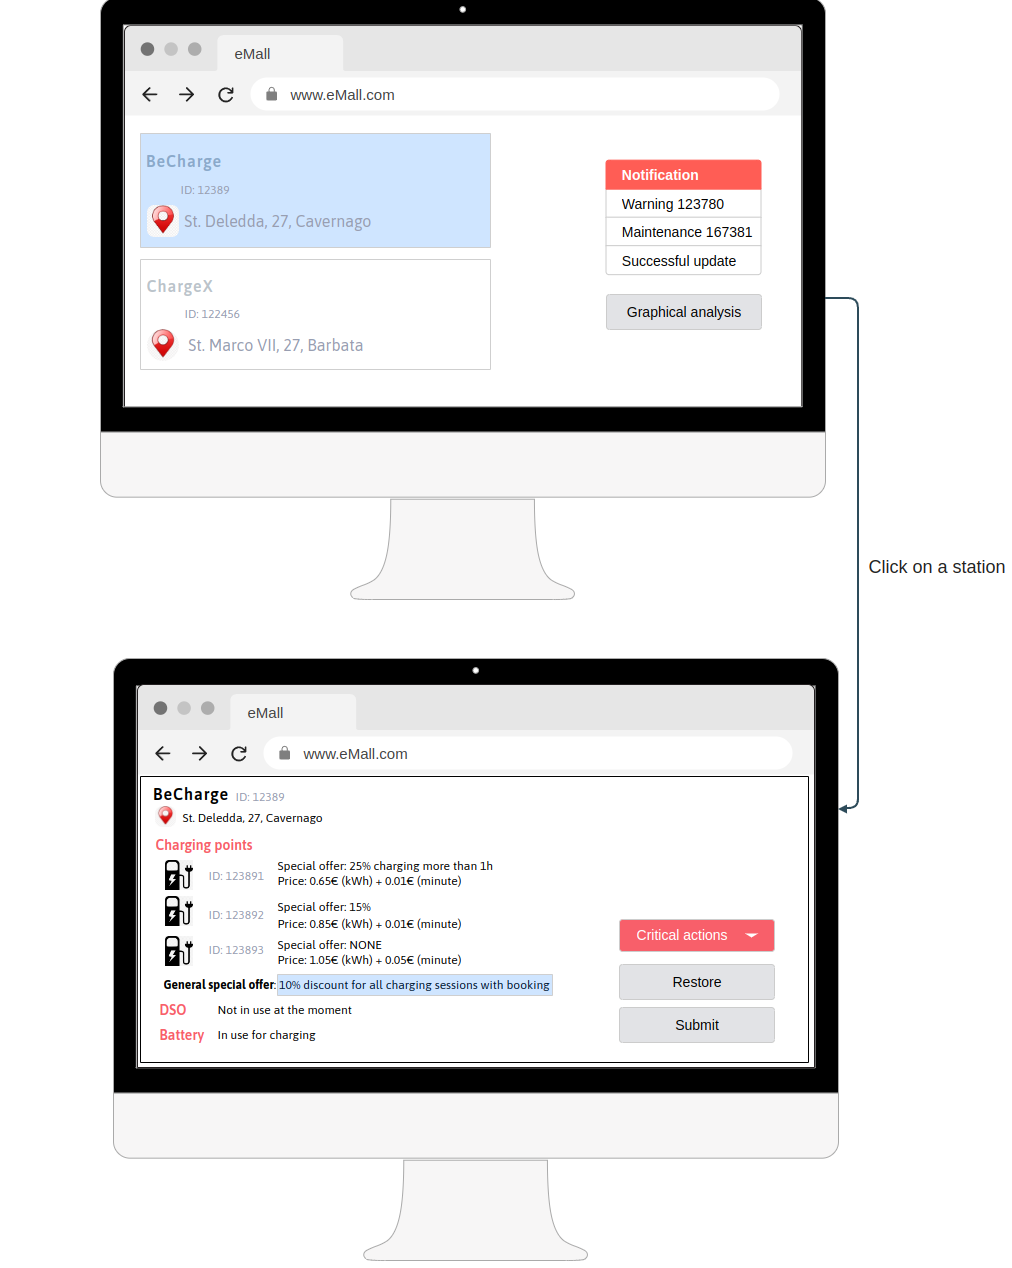
\includegraphics[width=0.75\textwidth]{Images/cp3/setPromotion.png}
    \caption{UI for visualizing the stations and adding a new promotion}
\end{figure}
In this minimal example of UI for the CPO we can see how the homepage allows to visualize the stations that the company is managing, and also presents the notifications sent by the system with a different specification and code, showing a precise communication type and the charging station it is related to. From the homepage the CPO can start the graphical analysis of the stations, can solve a notification and he can also select one of the stations to make some changes. In this case the CPO selects a station and the web app processes the request returning the page with the form related to the specific station. In the form a lot of data can be updated and added to manage the station and in this case the CPO adds a general special offer for the entire station and this will update the prices following the conditions of the promotion. Then the CPO submits the form and waits for a message that informs him of the success of the operation. From the station form is also possible to perform some critical actions, such as deleting the station, deleting a charging point or adding a new charging point.

\subsection{Update price}
\begin{figure}[H]
    \centering
    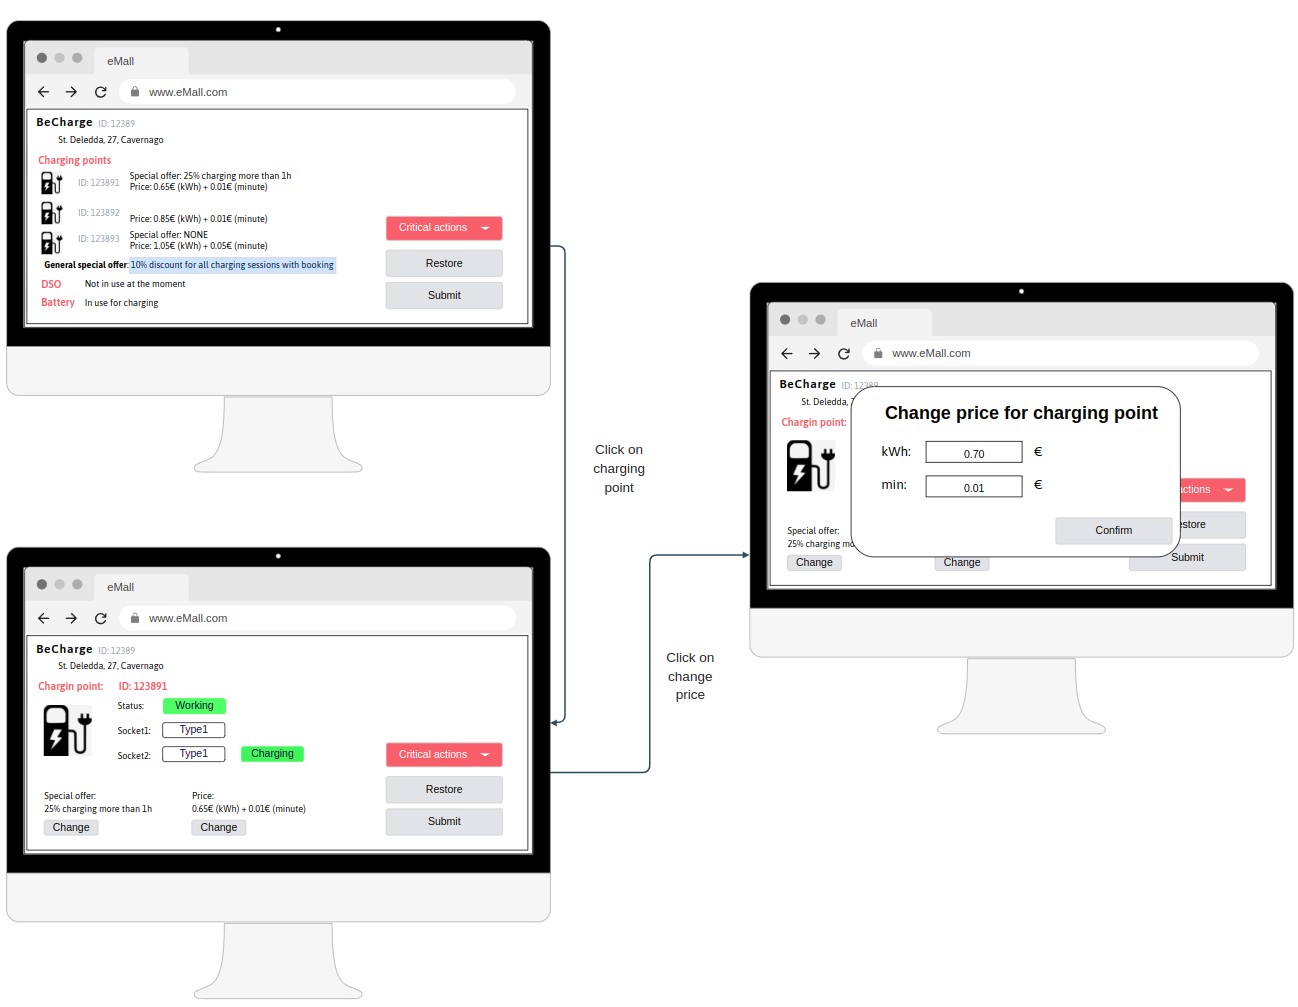
\includegraphics[width=1\textwidth]{Images/cp3/updatePrice.png}
    \caption{UI for updating the price of a charging point}
\end{figure}
From the homepage of a charging station the CPO can select a charging point to have a better view of its specifics. After clicking on charging point, the webapp loads a new page where the details of the device are shown. Specifically, the page shows the status of the charging point (working, off, not activated, etc.), its sockets with the respective type and if they are currently used for charging. In the section below the CPO can see the price set for the charging point and any special offer set on it. From this section the CPO, clicks the button to change the price and a popup comes up where he can insert the new price for the charging point. After entering the new price the CPO must confirm his entries by clicking on the Confirm button. Afterwards, the pop-up closes and the page of the charging point is reloaded with the new information. From this page the user can choose whether to confirm the changes, by clicking on the submit button, or undo the changes by clicking the restore button.

\subsection{Store energy in battery}
\begin{figure}[H]
    \centering
    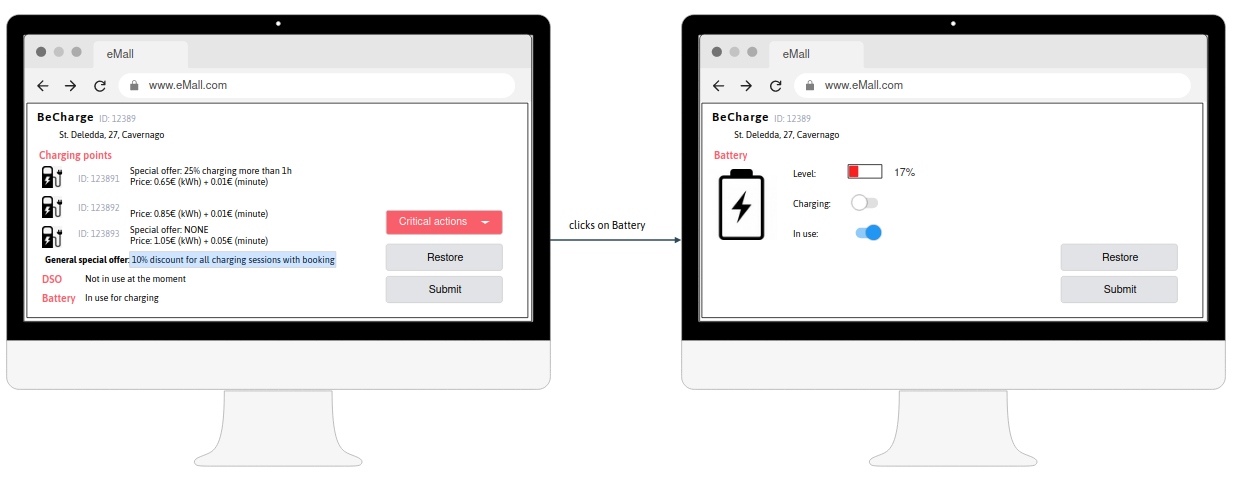
\includegraphics[width=1\textwidth]{Images/cp3/storeEnergyInBattery.png}
    \caption{UI for storing energy in battery}
\end{figure}
Same as before, the interaction with the CPO starts from the homepage of a charging station. From here the CPO can select the Battery text (if present), which will load the page for managing the battery of the charging station. This page shows the percentage of charge left in the battery, if the battery is charging and if the battery is currently in use. By clicking on the toggle \textit{Charging} the CPO can connect the battery to the grid and start charging it.

\subsection{Update DSO}
\begin{figure}[H]
    \centering
    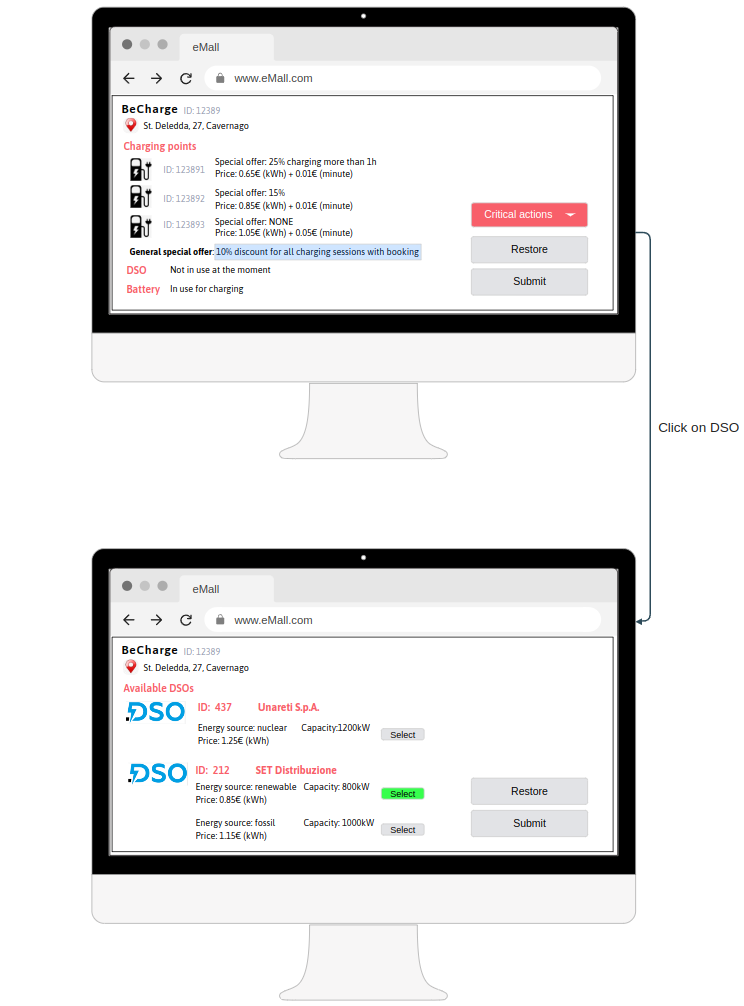
\includegraphics[width=0.73\textwidth]{Images/cp3/updateDSO.png}
    \caption{UI for updating the DSO of a charging station}
\end{figure}
Once on the charging station form is possible to select the DSO and update it or add it for the first time. Clicking on the DSO a new form is loaded in which the CPO can choose one from the available DSOs. For each one of them he can see the energy sources with the respective price and capacity. Is enough to select one DSO with the relative energy source and click the 'Submit' button. Then, a request will be sent to the CPMS part of the system, which will communicate through the DSO API with the external chosen DSO to update the contract, and will also save the new information on the DB. 

\subsection{Analyse stations}
\begin{figure}[H]
    \centering
    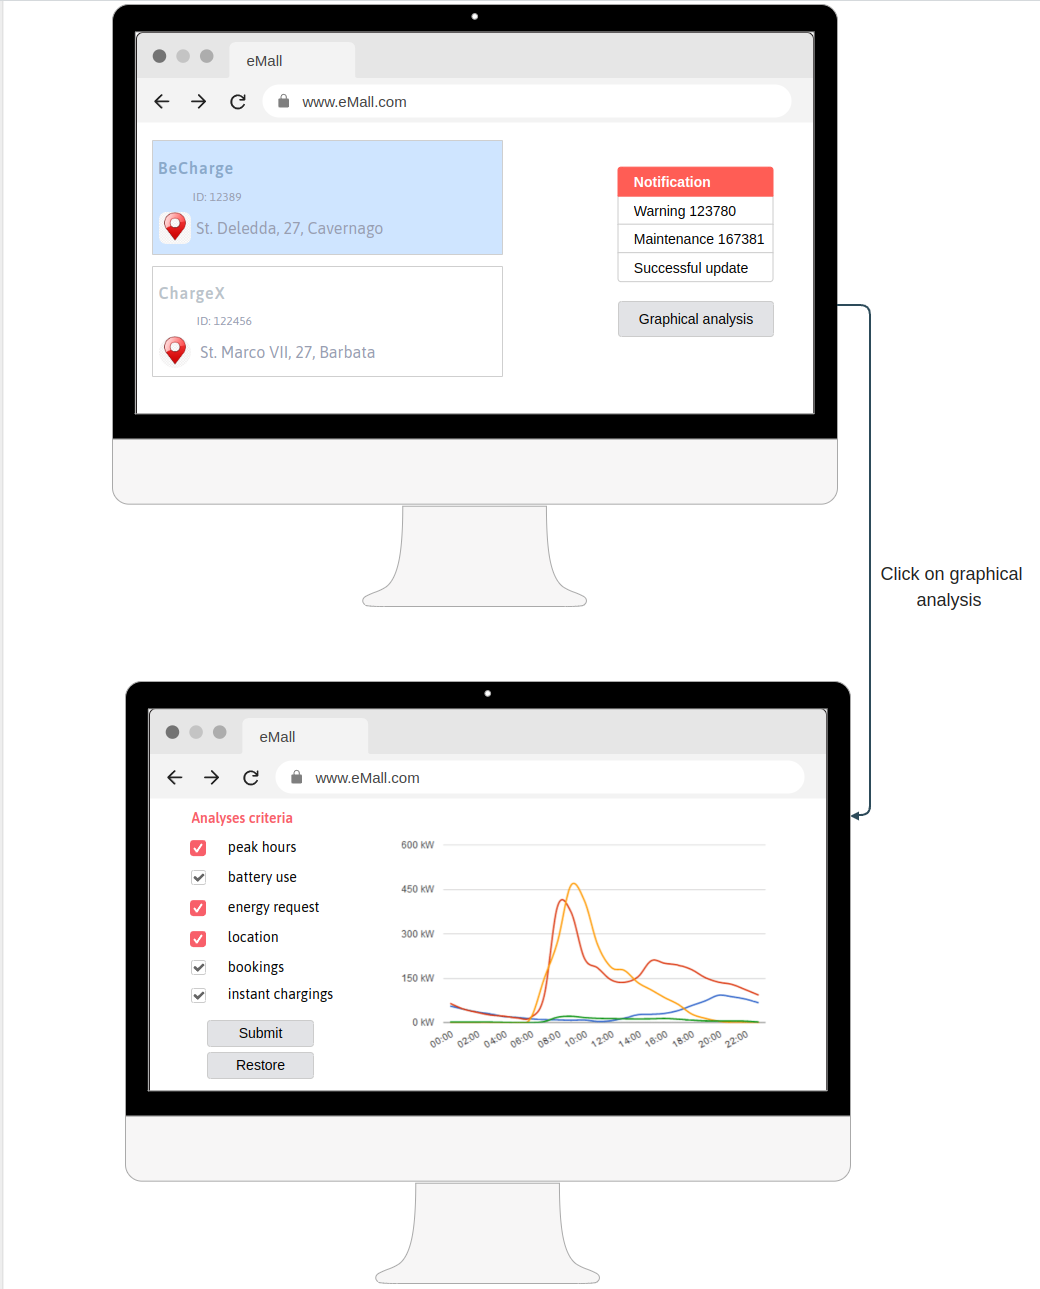
\includegraphics[trim={0.5cm 0cm 0cm 0.2cm},clip,width=0.75\textwidth]{Images/cp3/stationAnalysis.png}
    \caption{UI for analysing the stations}
\end{figure}
From the homepage, as explained before, the CPO can click the button 'Graphical analysis' and a new page is shown in which he has to select the criteria wanted for the analysis. Once submitted the choice, the eMall takes a few minutes to process the needed data and create a graphical view, that is shown reloading the page. In the reported UI we show an example of a graphical representation of the stations analyzed based on their location and on the energy request in order to identify the peak hours in which the service is used.  
\clearpage